\documentclass[8pt]{beamer}
\mode<presentation>
  {
    \usetheme{Pittsburgh}
    \setbeamercovered{transparent}
  }
\usefonttheme[]{serif}
%\usepackage[english,ukrainian]{babel}
\usepackage[english]{babel}
\usepackage[OT1,T2A]{fontenc}
\usepackage[cp1251]{inputenc} % ��������� ���������; ������ cp866nav.
\usepackage{amsfonts}
\usepackage{times}
%\usepackage[T1]{fontenc}
\usepackage{physics}
\usepackage{amsmath,amssymb}
\usepackage{graphicx}
%\usepackage[pdftex]{graphicx}
\usepackage{textcomp}
\usepackage{mathtext}
\usepackage{setspace}

\usepackage{epsf}
\usepackage{amsbsy}
%\usepackage{graphicx}

\mathchardef\ordinarycolon\mathcode`\:
\mathcode`\:=\string"8000
\begingroup \catcode`\:=\active
  \gdef:{\mathrel{\mathop\ordinarycolon}}
\endgroup

\newcommand{\no}{\nonumber}
\newcommand{\non}{\nonumber \\}
\newcommand{\ve}[1]{{\bf #1}}
\newcommand{\be}{\begin{equation}}
\newcommand{\ee}{\end{equation}}
\newcommand{\bea}{\begin{eqnarray}}
\newcommand{\eea}{\end{eqnarray}}
\newcommand{\sli}{\sum\limits}
\newcommand{\ili}{\int\limits}
%\newcommand{\lp}{\left (}
%\newcommand{\rp}{\right )}
%\newcommand{\lb}{\left [}
%\newcommand{\rb}{\right ]}
%\newcommand{\lbr}{\left \{}
%\newcommand{\rbr}{\right \}}
%\newcommand{\ld}{\left .}
%\newcommand{\rd}{\right .}
\newcommand{\vd}{\vec{d}}
\newcommand{\vR}{\vec{R}}
\newcommand{\vr}{\vec{r}}
\newcommand{\vk}{\vec{k}}
\newcommand{\vl}{\vec{l}}
\newcommand{\vp}{\vec{p}}
\newcommand{\vP}{\vec{P}}
\newcommand{\cM}{{\cal{M}}}
\newcommand{\cB}{{\cal{B}}}
\newcommand{\cV}{{\cal{V}}}
\newcommand{\rhok}{{\rho_{\vec{k}}}}
\newcommand{\rhomk}{{\rho_{-\vec{k}}}}
\newcommand{\etak}{{\eta_{\vec{k}}}}
\newcommand{\etamk}{{\eta_{-\vec{k}}}}
\newcommand{\nuk}{{\nu_{\vec{k}}}}

\setbeamertemplate{frametitle}{\raggedright \insertframetitle \par}
\begin{document}
\binoppenalty=10000
\relpenalty=10000

%-------------------------title------------------

\begin{frame}

\vspace{2cm}

\begin{center}
    \Large{\textbf{Grand partition function in collective variables}}
\end{center}

\vspace{2cm}

\begin{center}
    \textbf{R.V.~Romanik}
\end{center}
\end{frame}

%--------------------Table of Content----------------------

\begin{frame}
	\frametitle{Problem statement. Grand canonical ensemble.}
	
\begin{spacing}{1}
	
\begin{columns}
	\column{0.5\textwidth}
	
	\begin{equation*}
		\Xi=\sum_{N=0}^{\infty}\frac{z^N}{N!}Z_N
	\end{equation*}
	
	\begin{equation*}
		z = \frac{\exp(\beta\mu)}{\Lambda^3}
	\end{equation*}
	$\beta = kT$ -- the inverse temperature \\
	$\mu$ -- the chemical potential \\
	$\Lambda$ -- the de Broglie thermal wavelength 
	
	$Z_N$ -- the configuration integral:
	\begin{equation*}
		Z_N = \int\exp(-\beta U_N(\vb {r}^N)){\rm d}\vb{r}^N
	\end{equation*}
	
	$U_N({\vb r}^N)$ -- the potential energy of interparticle interaction
	
	\column{0.45\textwidth}
	
	
\end{columns}
\end{spacing}
	
\end{frame}

\begin{frame}
	\frametitle{Interaction potential}
	
	\begin{spacing}{1}
		
		\begin{columns}
			\column{0.5\textwidth}
			
			-- Interaction potential
			\begin{equation*}
				\label{interaction_decomp}
				U(r_{ij}) = \Psi(r_{ij}) + \Phi(r_{ij}),
			\end{equation*}
			
			 -- Potential energy of interaction
			\begin{equation*}
				U_N(\vb r^N) = \Psi_N(\vb r^N) + \Phi_N (\vb r^N) 
			\end{equation*}
			
			-- Short-range repulsion
			\begin{equation*}
				\Psi_N = \frac12 \underset{i\neq j}{\sum_{i=1}^N \sum_{j=1}^N} \Psi(r_{ij})
			\end{equation*}
			
			-- Long-range attraction
			\begin{equation*}
				\Phi_N = \frac12 \underset{i\neq j}{\sum_{i=1}^N \sum_{j=1}^N} \Phi(r_{ij})
			\end{equation*}
			
			
			\column{0.45\textwidth}
			- Hard spheres
			\begin{equation*}
				\Psi(r) = 
				\left\{
				\begin{array}{cc}
					\infty, \quad r\leq \sigma, \\
					0, \quad r > \sigma
				\end{array}
				\right.
			\end{equation*}	
			
			- Long-range
			\begin{equation*}
				\label{short-range-potential}
				\Phi(r) = \left\{
				\begin{array}{cc}
					0, \quad r \leq \sigma \\
					U_{\rm{Morse}}(r), \quad r > \sigma,
				\end{array}
				\right.
			\end{equation*}	
			
			- Morse potential
			\begin{equation*}
				U_{\rm{Morse}}(r) = \varepsilon \{{\rm e}^{-2\frac{r-R_0}{\alpha}}-2{\rm e}^{-\frac{r-R_0}{\alpha}}\}
			\end{equation*}	
		\end{columns}
	\end{spacing}
	
\end{frame}

\begin{frame}
	\frametitle{Microscopic particle density and collective variables}
	
	\begin{spacing}{1}
		
		\begin{columns}
			\column{0.5\textwidth}
			
			-- Microscopic particle density
			\begin{equation*}
				n(\vb r) = \sum_{j=1}^{N} \delta(\vb r - \vb r_j),
			\end{equation*}
			
			\begin{equation*}
				\int_V n(\vb r) d\vb r = N
			\end{equation*} 
			
			-- Fourier series
			\begin{equation*}
				n(\vb r) = \frac{1}{V} \sum_{\vb k} \hat{\rho}_{\vb k} e^{i\vb k \vb r}
			\end{equation*}
			
			-- Fourier components
			\begin{equation*}
				\label{def:rho_k}
				\hat{\rho}_{\vb k} = \sum_{j=1}^N\exp(-i\vb k \vb r_j), \quad \hat{\rho}_{\vb k = 0} = N. 
			\end{equation*}
			
			
			
			\column{0.45\textwidth}
			
			-- Collective variables
			\begin{equation*}
				\hat{\rho}_{\vb k} = \int\rho_{\vb k} J(\rho - \hat{\rho}) ({\rm d}\rho).
			\end{equation*}
			
			-- Jacobian of transformation
			\begin{equation*}
				J(\rho - \hat{\rho}) = \delta(\rho_0 - \hat{\rho}_0) \prod_{\vb k}' \delta(\rho_{\vb k}^c - \hat{\rho}_{\vb k}^c) \delta(\rho_{\vb k}^s - \hat{\rho}_{\vb k}^s),
			\end{equation*}
			
			\begin{equation*}
				({\rm d} \rho) = {\rm d}\rho_0 \prod_{\vb k}' {\rm d}\rho_{\vb k}^c {\rm d}\rho_{\vb k}^s.
			\end{equation*}
			
		\end{columns}
	\end{spacing}
	
\end{frame}

\begin{frame}
	\frametitle{Grand partition function in collective variables}
	
	\begin{spacing}{1}
		
		\begin{columns}
			\column{0.75\textwidth}
			-- Grand partition function (GPF)
			\begin{equation*}
				\Xi = \Xi_0 \int \exp(h\rho_0 - \frac12\sum_{\vb k}\alpha(k) \rho_{\vb k} \rho_{-\vb k}) \mathfrak{J}(\rho) ({\rm d} \rho)
			\end{equation*}
			
			$\Xi_0$ -- GPF of the reference system
			$h = \beta(\mu - \mu_0); \quad \alpha(k) = \frac{\beta\hat{\Phi}_{\vb k}}{V}$
			\hfill \break
			\hfill \break
			-- Jacobian function
			\begin{eqnarray*}
				\label{def:jacobian}
				\mathfrak{J}(\rho) &=& \frac{1}{\Xi_0}\sum_{N=0}^{\infty} \frac{z_0^N}{N!}\int \exp(-\beta\Psi_N(\vb r^N)) J(\rho - \hat{\rho}) {\rm d}{\vb r^N}
				\nonumber\\
				&=& \langle J(\rho - \hat{\rho}) \rangle_{RS}.
			\end{eqnarray*}
			
			
			\column{0.2\textwidth}
			
			
		\end{columns}
	\end{spacing}
	
\end{frame}

\begin{frame}
	\frametitle{Calculation of the Jacobian}
	
	\begin{spacing}{1}
		
		\begin{columns}
			\column{0.9\textwidth}
			-- Integral representation for $\delta-$functions
			\begin{equation*}
				\delta(\rho_0 - \hat{\rho}_0) \prod_{\vb k}' \delta(\rho_{\vb k}^c - \hat{\rho}_{\vb k}^c) \delta(\rho_{\vb k}^s - \hat{\rho}_{\vb k}^s) = \int \exp(2\pi{\rm i}\sum_{\vb k} (\rho_{\vb k} - \hat{\rho}_{\vb k}) \omega_{\bf k}) ({\rm d} \omega),
			\end{equation*}
			
			-- Cumulant (semi-invariant) expansion
			\begin{equation*}
				\mathfrak{J}(\rho) = \int \exp({\rm i} 2\pi \sum_{\vb k}\rho_{\vb k}\omega_{\vb k}) \tilde{\mathfrak{J}}(\omega) ({\rm d} \omega)
			\end{equation*}
			
			\begin{equation*}
				\tilde{\mathfrak{J}}(\omega) = \left< \exp(-{\rm i}2\pi \sum_{\vb k} \omega_{\vb k}\hat{\rho}_{\vb k}) \right>_{RS} 
				= \frac{(-{\rm i}2\pi)^n}{n!}\sum_{\vb{k}_1,\dotsc,\vb{k}_n}\mathfrak{M}_n(\vb k_1, \dotsc, \vb k_n) \omega_{{\vb k}_1}\dotsc \omega_{{\vb k}_n}
			\end{equation*}
			
			\column{0.1\textwidth}
			
			
		\end{columns}
	\end{spacing}
	
\end{frame}

\begin{frame}
	\frametitle{Cumulants}
	
	\begin{spacing}{1}
		
		\begin{columns}
			\column{0.9\textwidth}
			-- Definition (general formula):
			\begin{equation*}
				\label{def:cumulant}
				\mathfrak{M}_n(\vb k_1, \dotsc, \vb k_n) = \frac{1}{(-{\rm i}2\pi)^n} 
				\left(
				\frac{\partial^n \ln \tilde{\mathfrak{J}}(\omega)}{\partial\omega_{{\vb k}_1} \dotsc \partial\omega_{{\vb k}_n}}
				\right)_{\omega_{{\vb k}_i}=0}
			\end{equation*}
			
			-- It is shown that any cumulant $\mathfrak{M}_n$ can be represented as
			\begin{equation*}
				\mathfrak M_n(\vb k^n) = \langle N \rangle_0 \mathfrak m_n(\vb k^{n-1}) \delta_{\vb k_1 + \dotsc + \vb k_n}.
			\end{equation*}
			
			$\mathfrak{m}_n$ -- intensive quantity, can be interpreted as $n-$particle structure factor.
			
			
			\column{0.1\textwidth}
			
			
		\end{columns}
	\end{spacing}
	
\end{frame}

\begin{frame}
	\frametitle{Cumulants expressed via total correlation functions}
	
	\begin{spacing}{1}
		
		\begin{columns}
			\column{0.9\textwidth}
			\begin{equation*}
				\mathfrak{m}_1 = 1.
			\end{equation*}
			\begin{equation*}
				\label{m2}
				\mathfrak m_2(\vb k) = 1 + \rho \hat{h}^{(2)}(\vb k).
			\end{equation*}
			\begin{eqnarray*}
				\label{m3}
				\mathfrak m_3(\vb k_1, \vb k_2) &=& 1 +  \rho \big(\hat{h}^{(2)}(\vb k_1) + \hat{h}^{(2)}(\vb k_2) + \hat{h}^{(2)}(\vb k_1 + \vb k_2) \big)
				\nonumber\\ 
				&& + \rho^2 \hat{h}^{(3)}(\vb k_1, \vb k_2)
			\end{eqnarray*}
			
			\begin{eqnarray*}
				\label{m4}
				&& \mathfrak m_4(\vb k_1, \vb k_2, \vb k_3) =  1 
				\nonumber\\
				&& \quad{} + \rho \bigg(
				\sum_{l = 1}^3 \hat{h}^{(2)}(\vb k_l) +
				\sum_{\vb l = \left\{\substack{1,2 \\ 1,3 \\ 2,3} \right\} }  \hat{h}^{(2)} (\vb k_{l_1} + \vb k_{l_2})
				+ \hat{h}^{(2)} (\vb k_1 + \vb k_2 + \vb k_3)
				\bigg)
				\nonumber \\
				&&  \quad{} + \rho^2 \bigg(
				\sum_{\vb l = \left\{\substack{1,2 \\ 1,3 \\ 2,3 }\right\} }
				\hat{h}^{(3)}(\vb k_{l_1}, \vb k_{l_2})
				+ \sum_{\vb l = \left\{\substack{1,2,3 \\ 1,3,2 \\ 2,3,1}\right\} }
				\hat{h}^{(3)}(\vb k_{l_1} + \vb k_{l_2}, \vb k_{l_3})
				\bigg)
				\nonumber\\
				&& \quad{} + \rho^3 \hat{h}^{(4)} (\vb k_1, \vb k_2, \vb k_3)
			\end{eqnarray*}
			
			
			\column{0.1\textwidth}
			
			
		\end{columns}
	\end{spacing}
	
\end{frame}

\begin{frame}
	\frametitle{Some interesting properties of expressions for $\mathfrak{m}_n$}
	
	\begin{spacing}{1}
		
		\begin{columns}
			\column{0.9\textwidth}
			-- Bell number $B_n$ -- the total number of all terms contributing to $\mathfrak{m}_n$
			
			See \url{https://en.wikipedia.org/wiki/Bell_number}
			
			\hfill{} \break
			
			-- Stirling number of the second kind $S(n, k)$ -- the number of terms at the $k-$th power in $\rho$
			
			{ } \url{https://en.wikipedia.org/wiki/Stirling_numbers_of_the_second_kind}
			
			
			\column{0.1\textwidth}
			
			
		\end{columns}
	\end{spacing}
	
\end{frame}

\begin{frame}
	\frametitle{Graphical representations for $\mathfrak{m}_2$}
	
	\begin{spacing}{1}
		
		%\begin{columns}
		%	\column{0.9\textwidth}
			\begin{figure}[htbp]
				\includegraphics[width=0.45\textwidth,angle=0]{M2_as_function_of_k_at_different_eta2} \hfill
				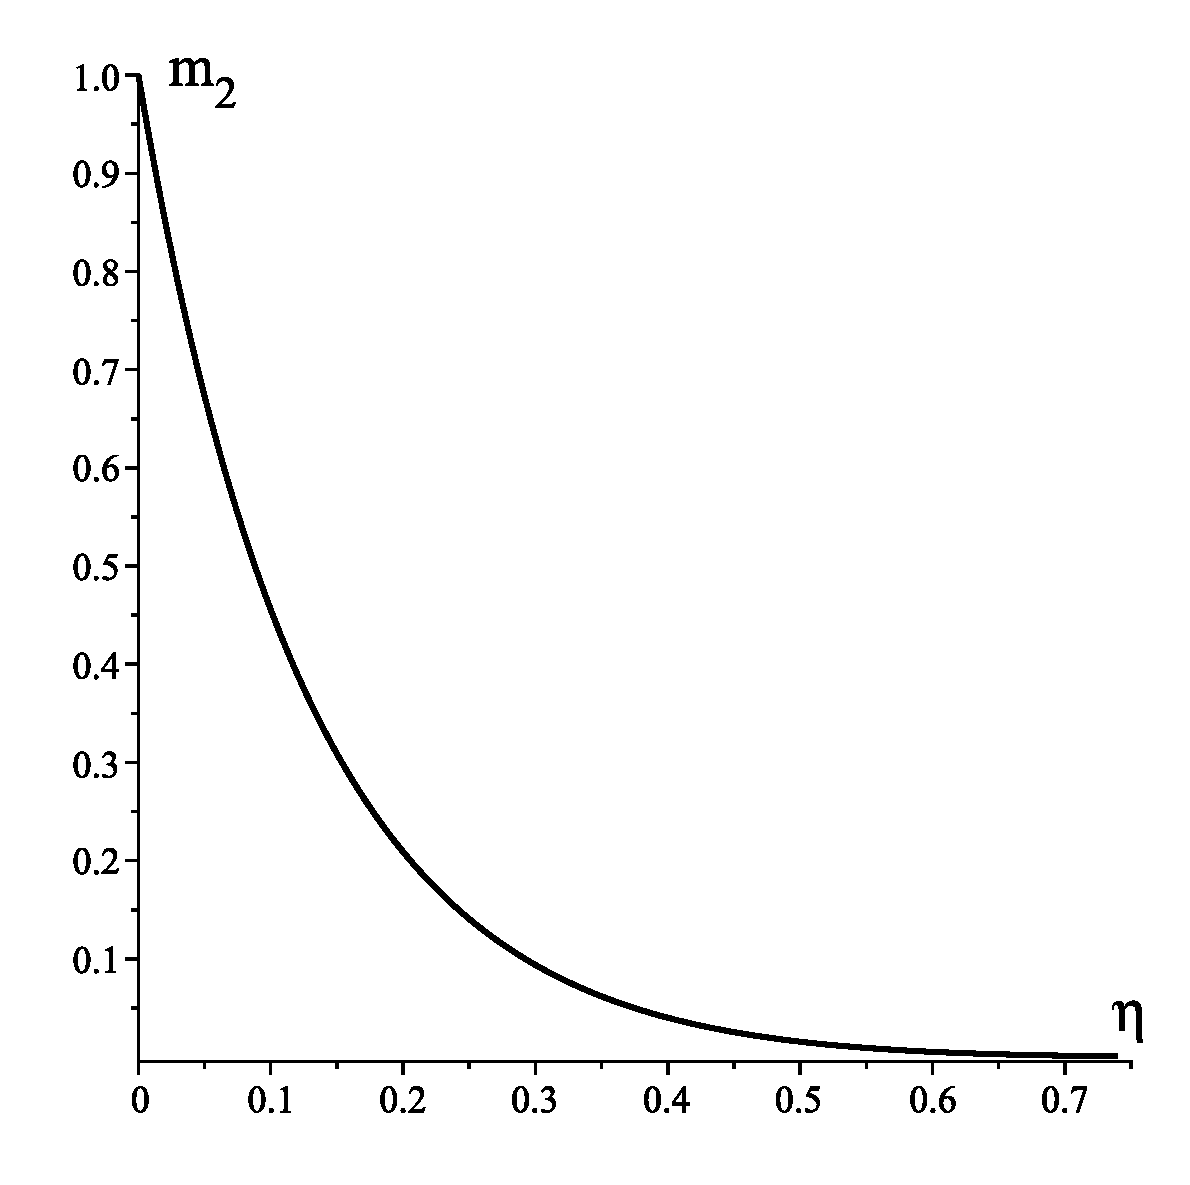
\includegraphics[width=0.45\textwidth,angle=0]{M2_as_function_of_eta_at_k_equals_0} \\
				\parbox{0.5\textwidth}{\caption{\label{m2_vs_k} Cumulant $\mathfrak{m}_2$ as a function of $k\sigma$ at different values of packing fraction $\eta$. 1 - $\eta = 0.05$, 2 - $\eta=0.1$, 3 - $\eta = 0.15$, and 4 - $\eta=0.2$.
				}} \hfill
				\parbox{0.45\textwidth}{\caption{\label{m2_vs_eta} Cumulant $\mathfrak{m}_2$ as a function of packing fraction $\eta$ at $\vb k = 0$
				}}
			\end{figure}
			
			
		%	\column{0.1\textwidth}
			
			
		%\end{columns}
	\end{spacing}
	
\end{frame}

\begin{frame}
	\frametitle{Graphical representations for $\mathfrak{m}_4$}
	
	\begin{spacing}{1}
		
		%\begin{columns}
		%	\column{0.9\textwidth}
		\begin{figure}[htbp]
			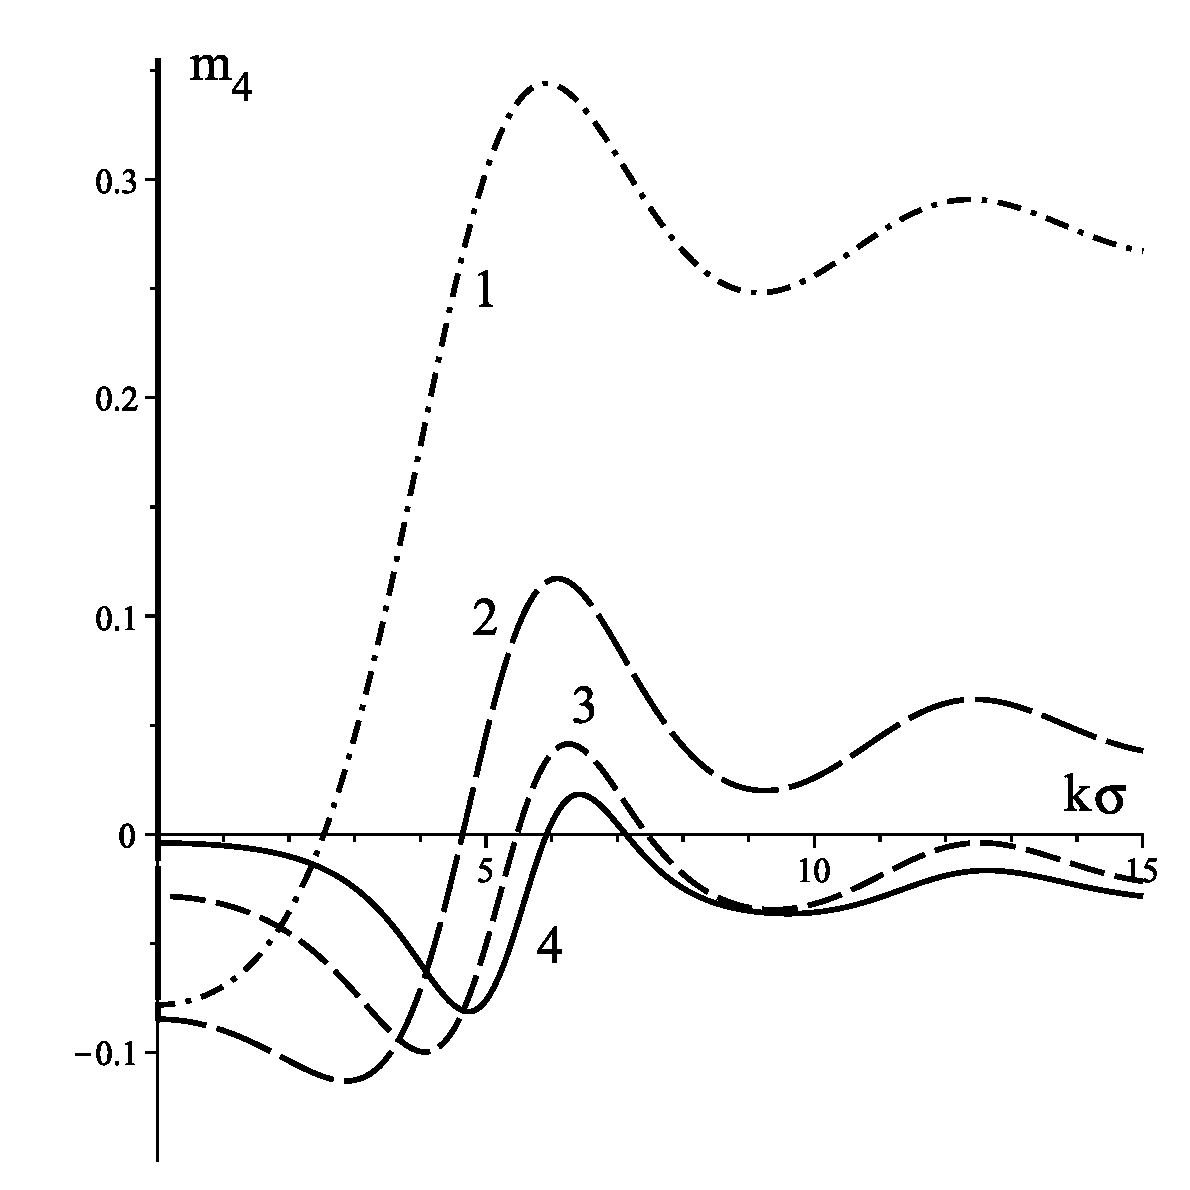
\includegraphics[width=0.45\textwidth,angle=0]{M4_as_function_of_k_at_different_eta} \hfill
			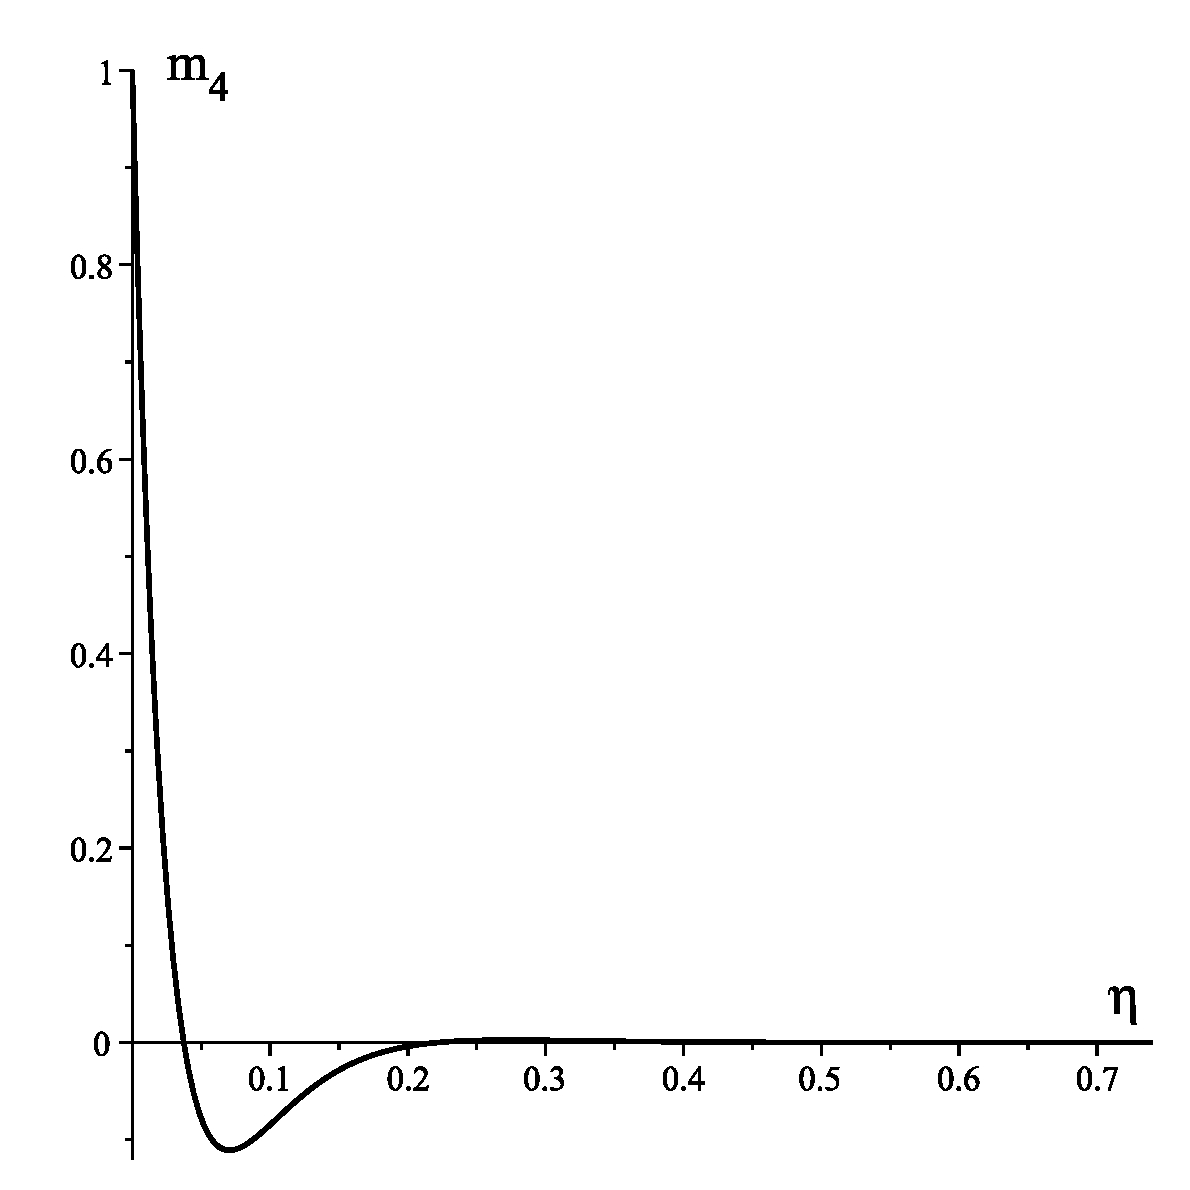
\includegraphics[width=0.45\textwidth,angle=0]{M4_as_function_of_eta_at_k_equals_0} \\
			\parbox{0.5\textwidth}{\caption{\label{m4_vs_k} Cumulant $\mathfrak{m}_4$ as a function of $k\sigma$ at different values of packing fraction $\eta$. 1 - $\eta = 0.05$, 2 - $\eta=0.1$, 3 - $\eta = 0.15$, and 4 - $\eta=0.2$.
			}} \hfill
			\parbox{0.45\textwidth}{\caption{\label{m4_vs_eta} Cumulant $\mathfrak{m}_4$ as a function of packing fraction $\eta$ at $\vb k = 0$
			}}
		\end{figure}

		
		
		%	\column{0.1\textwidth}
		
		
		%\end{columns}
	\end{spacing}
	
\end{frame}

\begin{frame}
	\frametitle{Total correlation functions}
	
	\begin{spacing}{1}
		
		%\begin{columns}
		%	\column{0.9\textwidth}

		
		
		
		%	\column{0.1\textwidth}
		
		
		%\end{columns}
	\end{spacing}
	
\end{frame}


\end{document} 